\documentclass[11pt]{article}

\usepackage{graphicx}
\usepackage{tikz}
\usepackage{pgfplots}



\begin{document}

\begin{center}
\bf MIE-PAA. Homework 1:\\[5mm]
\bf Solving the knapsack problem by brute force and simple heuristic\\[2mm]


\today
\end{center}

\section{Problem Statement.}
The \textbf{knapsack} problem or \textbf{rucksack} problem is a problem in combinatorial optimization: Given a set of items, each with a mass and a value, determine the number of each item to include in a collection so that the total weight is less than or equal to a given limit and the total value is as large as possible. It derives its name from the problem faced by someone who is constrained by a fixed-size knapsack and must fill it with the most valuable items.(wikipedia.org)\\

The knapsack problem should be solved in two ways: by a brute force and by the cost/weight ratio greedy heuristic. We are supposed to perform the experiments on sets of 50 instances of one size. \\

We are given instances of data to do the experiments. They are text files, the files are named \emph{knap n.inst.dat}, where n is the instance size. Each row describes one instance. Each instance is identified by (ID), the number of items (n) and the knapsack capacity (M) follow.

\section{Analysis of possible solutions.}

\textbf{Brute force algorithm}\\

Brute force algorithm is approach when we examine all possible combinations. For n-size instance we get $2^n$ combinations. After we construct a set:\\ $X = \{x_1, x_2, � ,x_n \}$, each $x_i$ will be 0 or 1.\\

We have \textbf{\emph{n}} - number of items, \textbf{\emph{M}} - the knapsack capacity and two sets \emph{\textbf{w}} = $\{w_1, ... ,w_n\}$ - that are weights of itmes and  \emph{\textbf{c}}= $\{c_1, ... ,c_n\}$ - costs of items.
And two conditions: the first one garantees that the knapsack is not overloaded, second one  give the maximum value of the knapsack. \\

$\sum_{i=1}^{n}w_ix_i = w_1x_1 + w_2x_2 + � + w_nx_n \leq M$ \\

$\sum_{i=1}^{n}cost_ix_i = cost_1x_1 + cost_2x_2 + � + cost_nx_n$ is max.\\

\textbf{Heuristic technique}\\

This technique differs from previous one. In this case we use cost/weight ratio. This rate is computed for each item from the list and after computing sorting is produced by this ratio.

As we do in the tutorials we take items with the highest ratio, until the first item that cannot be inserted is reached due to the fact that size is fixed. After we tried to find the smaller item that can fit.

\section{Brief description of solution, description of the algorithms used.}

\textbf{Brute force algorithm}\\

\section{The experimental results.}
\begin{tabular}{ |l|l| }
  \hline
  stuff & stuff \\ \hline
  stuff & stuff \\
  \hline
\end{tabular}
\begin{center}
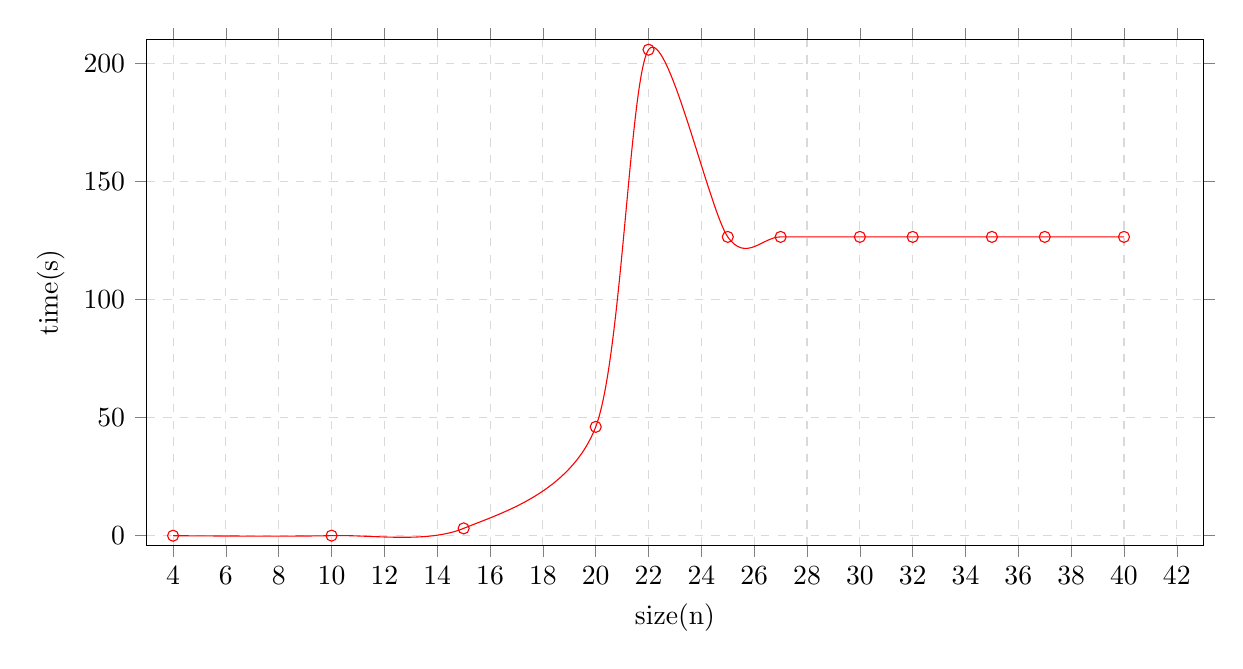
\begin{tikzpicture}
    \begin{axis}[
        width=15cm, height=8cm,     % size of the image
        grid = major,
        grid style={dashed, gray!30},
        %xmode=log,log basis x=10,
        %ymode=log,log basis y=10,
        xmin=3,     % start the diagram at this x-coordinate
        xmax=43,    % end   the diagram at this x-coordinate
        ymin=-4,     % start the diagram at this y-coordinate
        ymax=210,   % end   the diagram at this y-coordinate
        /pgfplots/xtick={0,2,...,60}, % make steps of length 5
     %   extra x ticks={23},
      %  extra y ticks={0.507297},
        axis background/.style={fill=white},
        ylabel=time(s),
        xlabel=size(n),
        tick align=outside]

\addplot[smooth,color=red,mark=o]
        plot coordinates {
            (4,0.00136)
            (10,0.02435)
            (15,3.10201)
	        (20,46.09)
	        (22,205.8)
	        (25,126.5236)
	        (27,126.5236)
	        (30,126.5236)
	        (32,126.5236)
	        (35,126.5236)
	        (37,126.5236)
	        (40,126.5236)
        };
    \end{axis}
\end{tikzpicture}
\end{center}

\section{Conclusions.}




\end{document}
